\documentclass[11pt]{beamer}
\usetheme{Madrid}
\usepackage[utf8]{inputenc}
\usepackage[german]{babel}
\usepackage[T1]{fontenc}
\usepackage{amsmath}
\usepackage{amsfonts}
\usepackage{amssymb}
\usepackage{graphicx}
\usepackage{multicol}
\usepackage{listings}
\usepackage{enumitem}
\usepackage{hyperref}
\usepackage[square,sort,comma,numbers]{natbib}
\usepackage{style/csharp}
\usepackage{minted}
\author{Florian Gehring}
\title{Vergleich zu C\#}
%\setbeamercovered{transparent} 
%\setbeamertemplate{navigation symbols}{} 
%\logo{} 
%\institute{} 
\date{18.06.2020} 
%\subject{} 

\setlist{parsep=3em}
\setlist{label=\textbullet}

\newmintedfile[csharpcode]{csharp}{
bgcolor=white,
linenos=true,
numberblanklines=true,
numbersep=3pt,
autogobble=true,
frame=leftline,
framerule=0.pt,
framesep=1mm,
funcnamehighlighting=true,
tabsize=4,
obeytabs=false,
mathescape=false
samepage=false, %with this setting you can force the list to appear on the same page
showspaces=false,
showtabs =false,
texcl=false,
fontsize=\small
}

\newmintedfile[javacode]{java}{
bgcolor=white,
linenos=true,
numberblanklines=true,
numbersep=3pt,
autogobble=true,
frame=leftline,
framerule=0.pt,
framesep=1mm,
funcnamehighlighting=true,
tabsize=4,
obeytabs=false,
mathescape=false
samepage=false, %with this setting you can force the list to appear on the same page
showspaces=false,
showtabs =false,
texcl=false,
fontsize=\small
}


\begin{document}
\setminted{linenos}
\begin{frame}
\titlepage
\end{frame}

%\begin{frame}
%\tableofcontents
%\end{frame}

% Hello World Frame
\begin{frame}{Hello, World!}
\csharpcode{Beispielcode/hello_world.cs}
%\lstinputlisting{Beispielcode/hello_world.cs}
Dieses und viele folgende Beispiele: \href{https://docs.microsoft.com/de-de/dotnet/csharp/tour-of-csharp/}{Tour of C\#}

\end{frame}


\begin{frame}{Geschichte}
\begin{itemize}
	\item Von Microsoft Entwickelt
	\item \glqq Direkter Konkurent\grqq{} zu Java
\end{itemize}
\end{frame}


\begin{frame}{Typsystem Allgemein}
	\begin{figure}
	\centering
		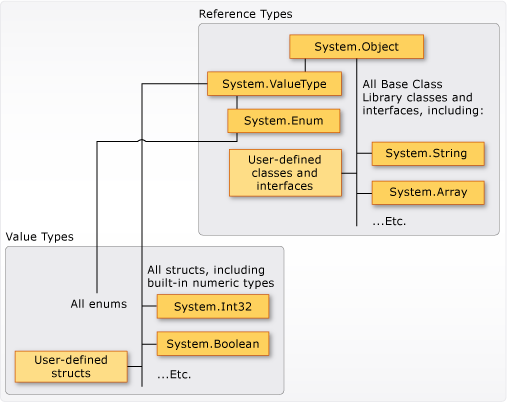
\includegraphics[width=0.7\textwidth]{bilder/value-reference-types-common-type-system.png}
		\caption{Type System in C\# \cite{progrguide}}
	\end{figure}
\end{frame}

\begin{frame}{Allgemeines Typsystem}
\begin{itemize}
% https://docs.microsoft.com/de-de/dotnet/csharp/programming-guide/types/
	\item Stark Typisiert
	\begin{itemize}
		\item jede Konstante, Variable und jeder Ausdruck hat einen Typ
	\end{itemize}
	\item CTS (Common Type System)
	\begin{itemize}
		\item \textbf{Jeder} Typ ist von \texttt{System.Object} (\texttt{object}) abgeleitet
	\end{itemize}

	\item Integrierte Typen
	\begin{itemize}
		\item \glqq Zahlen\grqq{}, \texttt{boolean}, \texttt{char}, \texttt{object}, \texttt{string}
	\end{itemize}
	\item Referenztypen / Werttypen
	\begin{itemize}
		\item \texttt{System.ValueType}
	\end{itemize}
	\item Benutzerdefinierte Typen
	\begin{itemize}
		\item \texttt{class, enum, struct}
	\end{itemize}
\end{itemize}
\end{frame}


\begin{frame}{Variablen Deklarationen}
\csharpcode[firstline=5, lastline=16]{Beispielcode/variable_declaration.cs}

%\lstinputlisting[linerange={1-2,5-16}]{Beispielcode/variable_declaration.cs}
\begin{itemize}
	\item \texttt{var} Keyword \cite{so_var_java}
	\item LINQ
\end{itemize}
\end{frame}


\begin{frame}{Werttypen}
\csharpcode[firstline=6, lastline=20, fontsize=\footnotesize]{Beispielcode/typesystem.cs}
System.Int32 \\ %\lstinputlisting[linerange={6-20}]{Beispielcode/typesystem.cs}
Int32 CompareTo(System.Object) Int32 CompareTo(Int32) ... \\
System.Int32 -> System.ValueType -> System.Object
\end{frame}


\begin{frame}{Werttypen - Vergleich Java}
	\begin{itemize}
		\item In Java: Integer $\neq$ int
		\item Zwar automatische Konvertierung, aber int ist kein Objekt
		\item Auskommentierte Zeilen führen zu Fehlern
	\end{itemize}
	\inputminted[firstline=9, lastline=15, linenos=true]{java}{Beispielcode/test/test.java}
	
\end{frame}


\begin{frame}{Zusammenfassung Typen}
% Create a line splitting two columns
\setlength{\columnseprule}{0.4pt}
\begin{multicols}{2}
	Java \\
	\begin{itemize}
		\item Primitive Typen nicht von \texttt{Object} abgeleitet
		\item Call-by-Value, Call-By-Reference
		\item Wrapper-Klasse \texttt{Integer} für \texttt{int}
	\end{itemize}

\columnbreak

	C\#\\
	\begin{itemize}
		\item Alles (auch \texttt{int}) von \texttt{object} abgeleitet
		\item Zahlen, boolean sind \glqq{}Werttype\grqq{}
		\item \texttt{int} kann mit \texttt{int?} Nullable gemacht werden
	\end{itemize}
\end{multicols}
\end{frame}


\begin{frame}{Klassen}

	\begin{itemize}
		\item Erben implizit von \texttt{object}
		\item  Enthalten: \texttt{constructors}, \textbf{\texttt{properties}}, \texttt{indexers}, \texttt{events}, \texttt{operators} and \texttt{destructors}
		 \item \texttt{sealed}-Modifier: Für die gesamte Klasse oder einzelne Methoden
	\end{itemize}

\end{frame}

\begin{frame}{Vererbung}
	Klassen \texttt{Base} und \texttt{Derived} mit den Methoden \texttt{ex1, ex2, ex3}.
	\csharpcode[fontsize=\tiny, firstline=1, lastline=28]{Beispielcode/classes.cs}
%	\csharpcode[fontsize=\tiny, firstline=13, lastline=28]{Beispielcode/classes.cs}
	% \lstinputlisting[basicstyle=\tiny,linerange={1-28}]{Beispielcode/classes.cs}
\end{frame}

\begin{frame}{Vererbung}
	\begin{columns}
		\begin{column}{0.7\textwidth}
				\csharpcode[firstline=31,lastline=48, fontsize=\footnotesize]{Beispielcode/classes.cs}
		\end{column}
		\begin{column}{0.3\textwidth}
		Ausgabe: \\
Base, example 1\\
Base, example 1\\
Derived, example 1\\
Base, example 2\\
Derived, example 2\\
Derived, example 2\\
Base, example 3\\
Base, example 3\\
Derived, example 3
			
		\end{column}
	

	\end{columns}

	% \lstinputlisting[basicstyle=\tiny,linerange={30-41}]{Beispielcode/classes.cs}

\end{frame}

\begin{frame}{Vererbung - Vergleich Java}
	
	\begin{itemize}
		\item Java: Alle Methoden sind virtuell
		\begin{itemize}
			\item Override wird mit \texttt{final} verhindert.
			\item Kein Äquivalent zu C\# \texttt{new}
		\end{itemize}
		\item Java: \texttt{@Override} Dekorator soll Code lesbarer machen
		\item In C\# Ingesamt expliziter als in Java
		\begin{itemize}
			\item Fokus auf Versionierung und Kompatibilität von Code
			\item Für interessierte: Interview mit C\# Chefdesigner \cite{interview_virtual}
		\end{itemize}
	\end{itemize}

\end{frame}

%---------------------
% 		Generics		-
%---------------------

\begin{frame}{Generics}

	\begin{enumerate}
		\item Syntax vorstellen
	\end{enumerate}

\end{frame}


\begin{frame}{Java Konzept: Type Erasure}
\begin{itemize}
	\item Java unterstützt auf Bytecode Ebene keine Generics
	\begin{enumerate}
		\item Keine generischen Typinformationen zur Laufzeit
	\end{enumerate}
	\item Generisches Argument wird durch möglichst spezifischen Typ ersetzt
	\begin{enumerate}
		\item \glqq Raw Types\grqq
	\end{enumerate}

\end{itemize}
\end{frame}



\begin{frame}{Type Erasure: Methoden}
	\begin{figure}
		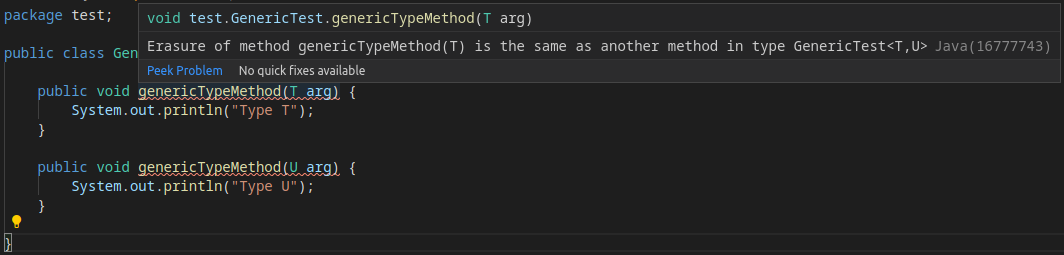
\includegraphics[width=\textwidth]{bilder/java_type_erasure.png}
	\end{figure}
	\csharpcode[firstline=2, lastline=8]{Beispielcode/GenericSort.cs}
\end{frame}

\begin{frame}{Type Erasure: Typen Generischer Klassen}
	Java
	\javacode[firstline=12, lastline=18]{Beispielcode/test/GenericTest.java}
	$C\#$
	\csharpcode[firstline=10, lastline=14]{Beispielcode/GenericSort.cs}
\end{frame}

\begin{frame}{Type Erasure: Objekt Instanziierung}
	Java
	\javacode[firstline=27, lastline=35]{Beispielcode/test/GenericTest.java}
	$C\#$
	\csharpcode[firstline=20, lastline=22]{Beispielcode/GenericSort.cs}
\end{frame}

\begin{frame}{Type Erasure: Statische Methoden}
	\begin{figure}
		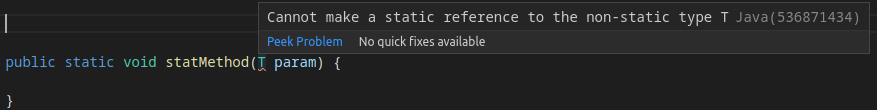
\includegraphics[width=\textwidth]{bilder/java_no_static_methods.png}
	\end{figure}
	
	$C\#$
	\csharpcode[firstline=25, lastline=40,fontsize=\tiny]{Beispielcode/GenericSort.cs}
\end{frame}

%-------------------------
% 		Delegates		-
%-------------------------

% Delegates
\begin{frame}{Delegates}
\begin{itemize}
 	\item \texttt{Delegates} sind Referenz\textbf{typen} (Objekte)
 	\item Sie kapseln die Funktionalität einer (anonymen) Methode
 	\item Die Methode wird mittels des Delegats aufgerufen
\end{itemize}
\csharpcode[firstline=3, lastline=4]{Beispielcode/delegates.cs}
	
\end{frame}
\begin{frame}{Delegates}
	Erstes Beispiel:
	\csharpcode[firstline=4, lastline=18]{Beispielcode/delegates.cs}
\end{frame}

\begin{frame}{Delegates}
	Initialisierung Möglich als: Methode mit Namen, Anonyme Methode und Lambda Funktion
	\csharpcode[firstline=35, lastline=41]{Beispielcode/delegates.cs}
\end{frame}

\begin{frame}{Delegates - Invocation List}
	\begin{itemize}
		\item  Eine Kombination von Delegaten ist möglich
		\item Methoden \texttt{TimesTwo (d1)} und \texttt{TimesThree (d2)} werden nacheinander mit 2 aufgerufen
		\begin{itemize}
			\item Delegatenaufruf gibt jetzt \texttt{void} zurück
		\end{itemize}
	\end{itemize}
	\csharpcode[firstline=20, lastline=33]{Beispielcode/delegates.cs}
\end{frame}

\begin{frame}{Delegates - Vergleich Java}
	\begin{itemize}
		\item Java: Functional Interfaces
		\begin{itemize}
			\item bestehend aus einer Funktion
			\item Automatisches Casten von Lambda-Ausdrücken
			\item \glqq Lambda expressions let you express instances of single-method classes more compactly.\grqq
			\item \texttt{@FunctionalInterface} Annotation		
		\end{itemize}
		\item Wieder weniger explizit
		\item Man sieht nicht am Datentyp, dass es sich um eine Funktion handelt
		\item Vgl. Vortrag letztes Mal: \glqq Real Function Types\grqq
	\end{itemize}
\end{frame}



%-------------------------
% 		Quellen	    		-
%-------------------------

\begin{frame}{Quellen}
\begin{thebibliography}{99}
\fontsize{6pt}{7.2}\selectfont
	\bibitem{progrguide}"Programming Guide C\#", \url{https://docs.microsoft.com/de-de/dotnet/csharp/programming-guide/}, 05.06.2020
	\bibitem{spec_csharp} C\# Language Specification, \url{https://docs.microsoft.com/de-de/dotnet/csharp/language-reference/language-specification/introduction}, 05.06.2020
   \bibitem{intro_csharp}Introduction to C\#, \url{https://docs.microsoft.com/de-de/dotnet/csharp/language-reference/language-specification/introduction}, 06.06.2020

 \bibitem{so_var_java}'"What is the equivalent of the C\# 'var' keyword in Java?"', 
 \url{https://stackoverflow.com/a/49598148}, 05.06.2020
 \bibitem{interview_virtual}'Interview with C\# Designer', \url{https://www.artima.com/intv/nonvirtual.html}, 06.06.2020
 \bibitem{java_generics} 'Java Generics' \url{https://docs.oracle.com/javase/tutorial/java/generics/restrictions.html}, 08.06.2020
 \bibitem{blog_vgl_generics} 'Blogpost C\# / Java Generics', \url{http://www.jprl.com/Blog/archive/development/2007/Aug-31.html}, 09.06.2020
\end{thebibliography}
\end{frame}
\end{document}
